
%%%%%%%%%%%%%%%%%%%%%%%%%%%%%%%%%%%%%%%%%%%%%%%%%%%%%%%%%%%%%%%%%%%%%%%
%                            First Chapter                            %
%               State of the Art of Posture Generation                %
%%%%%%%%%%%%%%%%%%%%%%%%%%%%%%%%%%%%%%%%%%%%%%%%%%%%%%%%%%%%%%%%%%%%%%%

\chapter{State of the Art of Posture Generation}
\label{cha:state_of_the_art_of_posture_generation}

\nomenclature[z-PG]{PG}{Posture Generation}
\nomenclature[z-IK]{IK}{Inverse Kinematics}
\nomenclature[z-DoF]{DoF}{degrees of freedom}
\nomenclature[x-I]{$\mathbb{I}_n$}{Matrix identity of dimension $n$}
\nomenclature[x-w]{$\wedge$}{cross product}
\nomenclature[z-mbg]{mbg}{Multibody Graph}
\nomenclature[a-F]{F}{a frame}
\nomenclature[a-W]{W}{the world frame}
\nomenclature[a-w]{w}{a wrench or a force}
\nomenclature[a-f]{f}{a force resultant}
\nomenclature[a-m]{m}{a force moment}


\graphicspath{{Chapter1-PG/Figs/Vector/}{Chapter1-PG/Figs/}}

\section{List of contributions}
\begin{itemize}
  \item Generalities, introduction
  \item Presentation of the existing methods
  \item From Inverse Kinematics to Generalized IK/posture Generation/pose estimation (addition of articular limits, forces, stability etc).
  \item Topology of the parametrization space (Free-flyer, q, f, other)
  \item Formulation as a non-linear constrained optimization problem
  \item Adrien \& Karim's formulations
  \item Formulation of several types of cost/constraints
  \begin{itemize}
    \item Contact with planar surface
    \item Collision avoidance
    \item Auto-Collision avoidance
    \item Static equilibrium: Newton/CoM projection
    \item Forces in friction cones
    \item Articular limits
    \item Torque limits
    \item Torque minimization
    \item Goal Posture
  \end{itemize}
  \item Reasons why it is not enough and why we needed a new PG
    \begin{itemize}
      \item Having an easier way to formulate problems
      \item Avoid having to de some gymnastic to remain on manifolds
      \item Automatic variable management
      \item Robustness
    \end{itemize}
  \item Utilization of posture generation in planning
\end{itemize}

\section{Problem Definition}
\label{sec:problem_definition}

We consider the problem where we have a robotic system and we want to have it do some tasks, like for example to make a contact between a point on a body of the robot and a point of the environment.
This contact task can be modelized as a simple equality.
We denote $q$ the joint parameters of the robot, $g(q)$ is the 3D position of the point of interest on the robot and $P$ is the point of the environment.
Then our problem comes down to finding a configuration $q^*$ such that $f(q^*) = P$.
For complicated robots like humanoids, the equations describing its kinematics are quite complicated, and the presence of angular joints in the robotic system imply the non-linearity of those equations.
In the general case, even for simple tasks, a closed form solution of the problem does not exist.

We denote $\mathcal{C}$ the configuration space of our robotic system. It is the manifold in which $q$ lives. The dimension of $\mathcal{C}$ for a single robot in equal to the number of degrees of freedom of the robot. Note that if all the joints of the robot are actuated, this is the number of motors of the robot. And if the robot has a free-floating basis (is not fixed) then the position in $\mathcal{R}^3$ and rotation in $SO(3)$ of its basis are to be added to $q$.

We can formulate that problem as follows:

\begin{equation}
  \text{find}\ q\in\mathcal{C}\ \text{such that}\ g(q)=P
\end{equation}

The space of solution of this problem is a submanifold of $\mathcal{C}$ of lower dimension that we call ${\mathcal{C}}_F$ the feasible configuration space (which can be empty).

In addition to the equality constraint abovementioned, the problem can feature some inequality constraints.
For example, each joint variable can be limited to a certain range of value: $\forall i,\ q_i\in [q_i^-,\ q_i^+]$. Then the problem becomes a combination of equality and inequality constraints, and can be written as:
\begin{equation}
  \text{find}\ q\in\mathcal{C}\ \text{such that}\left\{
  \begin{array}{l}
    g(q)=P \\
    \forall i,\ q_i^- \leq q_i \leq q_i^+
  \end{array}
  \right.
\end{equation}

Finally, we can also require finding the point of $\mathcal{C}_F$ that minimizes a criterion, such as the distance to a goal posture $q_0$ for example.
Our problem becomes:

\begin{equation}
  \left\{
  \begin{array}{l}
    \min\limits_{q\in\mathcal{C}}{\|q-q_0\|_2}\\
    \text{ s.t. }
    \left\{
    \begin{array}{l}
      g(q)=P\\
      \forall i,\ q_i^- \leq q_i \leq q_i^+
    \end{array}
    \right.
  \end{array}
  \right.
\end{equation}

This type of problem is called a nonlinear constrained optimization problem and can be formulated in a more generic fashion as:

\begin{equation}
\label{eq:optim_form_PG}
  \left\{
  \begin{array}{l}
    \min\limits_{x\in\mathcal{C}}{f(x)}\\
    \text{ s.t. }
    \left\{
    \begin{array}{l}
      c_i(x) = 0,\ \forall i\in{E}\\
      c_i(x) \geq 0,\ \forall i\in{I}\\
    \end{array}
    \right.
  \end{array}
  \right.
\end{equation}

Where $x$ is the optimization variable in space $\mathcal{C}$ that we want to find, such that it minimizes the cost function $f(x)$ while satisfying all the equality constraints $c_i(x) = 0,\ \forall i\in{E}$ and inequality constraints $c_i(x) \geq 0,\ \forall i\in{I}$

Such problems can be solved by a Non-linear optimization solver.
In Appendix~\ref{chapter:optimization}, we present some principles of nonlinear optimization in unconstrained and constrained cases.
Several off-the-shelf solvers are available and have been widely used in for solving robotics problems.
The CFSQP solver~\cite{cfsqp:manual} was used in~\cite{escande:iros:2009} and~\cite{escande:ras:2013} where thousands of HRP-2 posture generation queries were made to explore the feasible space.
The IPOPT solver has been used in~\cite{vaillant:humanoids:2014},~\cite{vaillant:autonomousrobots:2016},~\cite{bouyarmane:ar:2012} where the posture generator had been extended to handle multi-robot problems and more complex and various contact models.
In this thesis, we use those off-the-shelf solvers a little in the beginning and later we tackle the development of our own non-linear optimization solver.

From this point forward, we formulate and solve posture generation problems as nonlinear constrained optimization problem. And in the next sections, we focus on the formulating several robotics constraints and cost function in the formalism of nonlinear optimization.


\section{Problem Formulation}
\label{sec:pg_formulation}

\subsection{Forward Kinematics}
\label{sub:forward_kinematics}

In this section, we present a formulation of robotic systems that allows specifying most of the typical constraints encountered in robotics problems.

We consider a robotic system made of $n_B$ bodies and $n_J$ joints.
The global structure of the robot is described by an ordered graph called $mbg$ multi-body graph.
The base body (World) has index $0$ and other bodies get different positive integer index, we denote the body of index $i$, $B_i$. And $B_0$ can be called $B_W$.
Each body $B_i$ has its reference frame $F_i$ attached to it.
$F_0$ or $F_W$ denotes the World frame.
Bodies are linked together by joints that also are indexed by positive integers, we denote the joint of index $i$, $J_i$, and the body that comes after it is $B_i$.
Each joint defines the relation between its predecessor and successor bodies, for joint $J_i$ they are respectively denoted $pred(i)$ and $i$, and $B_{pred(i)}$ is called the parent body of $B_{i}$.
We denote $\lambda(j)$ the index of the parent body of $B_j$.
The number of degrees of freedom of $J_i$ is denoted $dof^J_i$ and the number of degrees of freedom of the whole robot is denoted $dof$.
Figure~\ref{fig:mbg} illustrates this numbering system for a simple robot with 4 joints and 5 bodies (including the basis)

\begin{figure}
  \centering
  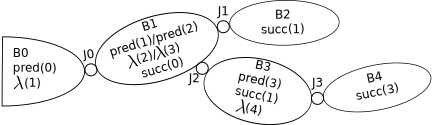
\includegraphics[width=0.7\textwidth]{mbg.pdf}
  \caption{MultiBody graph}
\label{fig:mbg}
\end{figure}

The geometric relations between bodies and joints are described through transformations between their reference frames. Each body $B_i$ has a reference frame $F_i$ attached to it. Transformations are described in the Spacial Vector Algebra chapter of `Rigid Body Dynamics Algorithm' by Roy Featherstone~\cite{featherstone:book:2007}.

Let A and B be Cartesian frames with origins O and P respectively. Let $\mathbf{t}$ be the coordinate vector expressing $\overrightarrow{OP}$ in A. And $\mathbf{R}$ be the rotation matrix that transforms 3D vectors from A to B coordinates.
The transformation from A to B for a motion vector is defined by:
\begin{equation}
  {}^B X_A =
  \begin{pmatrix}
    \mathbf{R} & \mathbf{0} \\
    -\mathbf{R}\hat{\mathbf{t}} & \mathbf{R} \\
  \end{pmatrix}
\end{equation}
Its inverse is:
\begin{equation}
  {{}^B X_A}^{-1} = {}^A X_B =
  \begin{pmatrix}
    \mathbf{R}^T & \mathbf{0} \\
    \hat{\mathbf{t}}\mathbf{R}^T & \mathbf{R}^T \\
  \end{pmatrix}
\end{equation}
The transformation from A to B for a force vector is defined by:
\begin{equation}
  {}^B X_A^* =
  \begin{pmatrix}
    \mathbf{R} & -\mathbf{R}\hat{\mathbf{t}} \\
    \mathbf{0} & \mathbf{R} \\
  \end{pmatrix}
\end{equation}
Its inverse is:
\begin{equation}
  {}^B X_A^{-*} = {}^A X_B^* =
  \begin{pmatrix}
    \mathbf{R}^T & \hat{\mathbf{t}}\mathbf{R}^T \\
    \mathbf{0} & \mathbf{R}^T \\
  \end{pmatrix}
\end{equation}

%Each joint $J_i$ is defined in the reference frame of its predecessor body by a static transformation $X^x_i = \{\mathbf{R}^x_i, \mathbf{t}^x_i\}$ from the base of the body to the base of the joint.
Each joint $J_i$ is defined by a static transformation $X^x_i = \{\mathbf{R}^x_i, \mathbf{t}^x_i\}$ between the reference frame of its predecessor body and its own reference frame.
Each joint $J_i$ is associated with a motion subspace which representation matrix is denoted $\mathbf{S}_i$. Each column of $\mathbf{S}_i$ described a degree of freedom of $J_i$ its upper part for the rotations and lower for translations.
\begin{equation}
  \mathbf{S}_i =
  \begin{pmatrix}
    S^R_{i,0} & \cdots &
    S^R_{i,j} & \cdots &
    S^R_{i,dof} \\
    S^t_{i,0} & \cdots &
    S^t_{i,j} & \cdots &
    S^t_{i,dof}
  \end{pmatrix}
\end{equation}

For a given joint configuration $q$, the transformation due to the joint $J_i$ current configuration from its reference frame to the reference frame of its successor body is denoted \\$X^J_i (q) = \{\mathbf{R}^J_i (q), \mathbf{t}^J_i (q)\}$.

The transformation between $B_{\lambda(i)}$ and $B_i$ is denoted $X^{PtS}_i (q) = \{\mathbf{R}^{PtS}_i, \mathbf{t}^{PtS}_i\}$ (PtS stands for `Parent to Son') can then be computed as:
\begin{equation}
  {X}^{PtS}_i (q) = {}^{i}X_{\lambda (i)} (q) = X^J_i (q) X^x_i
  \label{eq:PtS}
\end{equation}

Let $\kappa (i) =\{0, i_1, i_2 \ldots i\}$ be the list of indexes of successive joints going from $B_W$ to $B_i$.
It can easily be computed by adding iteratively the parent of the current body:

\begin{algorithm}
  \caption{Joint Path to $B_i$}
\label{JP}
\begin{algorithmic}
  \State{$j \leftarrow i$, $\kappa(i)=[i]$}
  \While{$j \neq 0$}
  \State{$j \leftarrow \lambda(j)$}
  \State{$\kappa(i) \leftarrow [\kappa(i),\ j]$}
  \EndWhile{}
\end{algorithmic}
\end{algorithm}

The transformation from the World base to $B_i$ is denoted \\ ${}^i X_W (q) = \{{}^i \mathbf{R}_W (q), {}^i \mathbf{t}_W (q)\}$.
The formula~\ref{eq:PtS} can be used iteratively on every body of the robot to obtain the expression of ${}^i X_W (q)$.

We obtain the full expression of ${}^i X_W$ as:
\begin{equation}
  {}^i X_W (q) = \prod_{j\in\kappa (i)}X^J_j (q) X^x_j = \prod_{j\in\kappa (i)}\ {}^j X_{\lambda (j)}
  = {}^i X_{\kappa (1)}\ ^{\kappa (1)}X_{\kappa (2)} \dots ^{\kappa (\text{end}-1)}X_{W}
\end{equation}

Which can be computed recursively by a Forward Kinematics algorithm:

\begin{algorithm}
  \caption{Forward Kinematics}
\label{FK}
\begin{algorithmic}
  \For{$i = 0:n_J$}
  \If{$\lambda (i) \neq -1$} ${}^i X_W = {}^i X_{\lambda (i)}\ ^{\lambda (i)}X_W$
  \Else$\ {}^i X_W = X^{PtS}_i$
  \EndIf{}
  \EndFor{}
\end{algorithmic}
\end{algorithm}

In the following section, we provide some detailed description of how to compute $X_J (q)$ for a variety of useful joints.
Using the joint descriptions and the Forward Kinematics algorithm, we are able to explicit a relation between $q$ the joint parameters of the robot and the 3D position and orientation of  any geometric quantity defined in the reference frame of a body of the robot.
Given a transformation ${}^p X_i$ defined in the frame of $B_i$, its value in the world frame is given by ${}^p X_W (q) = {}^p X_i\ {}^i X_W (q)$

\subsection{Joints formulations}
\label{sub:joints_formulations}

The entire geometry of our system is described by the list of static transformations $X^x_j$ and of joint transformations $X^J_j (q)$.
In this section, we explicit the descriptions and formulations of several useful joints.

Let us consider a joint $J$ that governs the transformation between two frames $F_1=\{O_1, x_1, y_1, z_1\}$ and $F_2=\{O_2, x_2, y_2, z_2\}$.
The most common type of joint encountered in robotics systems is the revolute joint, that allows a rotation around a fixed axis.
If $J$ is a revolute joint around the axis $(O_1,z_1)$ with parameter $q$, its motion subspace, rotation and translation are as follows:

\begin{table} [ht]
\centering
\begin{tabular}{cccc}
  \toprule
  Joint type & $S$ & $Rotation$ & $translation$ \\
  \midrule
  Revolute $(O_1,z_1)$
  &
  $\begin{pmatrix}
    0 \\ 0 \\ 1 \\ 0 \\ 0 \\ 0
  \end{pmatrix}$
  &
  $\begin{pmatrix}
    1 & 0 & 0 \\
    0 & \cos (q) & \sin (q) \\
    0 & -\sin (q) & \cos (q) \\
  \end{pmatrix}$
  &
  ${\bf 0}_{3\times1}$
  \\
  \bottomrule
\end{tabular}
\end{table}

Similar formulas can be devised for rotations around any other axis, provided that $R$ describes the rotation of angle $q$ around that axis.

In the case of a prismatic joint, all rotations are blocked, and only one translation along a given axis is allowed.
A prismatic joint along $x_1$ is described by the following formulas:

\begin{table} [ht]
\centering
\begin{tabular}{cccc}
  \toprule
  Joint type & $S$ & $Rotation$ & $translation$ \\
  \midrule
  Prismatic $(x_1)$
  &
  $\begin{pmatrix}
    0 \\ 0 \\ 0 \\ 1 \\ 0 \\ 0
  \end{pmatrix}$
  &
  ${\bf 1}_{3\times3} $
  &
  $\begin{pmatrix}
    q \\ 0 \\ 0
  \end{pmatrix}$
  \\
  \bottomrule
\end{tabular}
\end{table}

Planar joints are also frequently used in robotics.
A planar joint describes a plan sliding on another plan, assuming that the normal to both plans is $z_1 = z_2$ this type of joint allows free rotation of $F_2$ around $z_1$ and translations along $x_1$ and $y_1$. We denote $q = \{q_1, q_2, q_3\}$ the joint parameters, $q_1$ corresponding to the rotation and $q_2,\ q_3$ to the translations. We get:

\begin{table} [ht]
\centering
\begin{tabular}{cccc}
  \toprule
  Joint type & $S$ & $Rotation$ & $translation$ \\
  \midrule
  Planar $(z_1)$
  &
  $\begin{pmatrix}
    0 & 0 & 0 \\ 0 & 0 & 0 \\ 1 & 0 & 0 \\ 0 & 1 & 0 \\ 0 & 0 & 1 \\ 0 & 0 & 0
  \end{pmatrix}$
  &
  $\begin{pmatrix}
    1 & 0 & 0 \\
    0 & \cos(q_1) & \sin(q_1) \\
    0 & -\sin(q_1) & \cos(q_1) \\
  \end{pmatrix}$
  &
  $\begin{pmatrix}
    \cos(q_1)q_2 - \sin(q_1)q_3 \\ \sin(q_1)q_2 + \cos(q_1)q_3 \\ 0
  \end{pmatrix}$
  \\
  \bottomrule
\end{tabular}
\end{table}

A spherical joint blocks all translations and allows all rotations. This joint must be parameterized by a 3D rotation. The space of 3D rotations $SO(3)$ can be represented in many different ways.
The simplest and most intuitive way to parameterize $SO(3)$ is to use Euler Angles.
It comes down to decomposing the 3D rotation into a succession of three 1D rotations around different axes.
For example, the roll, pitch, yaw is a succession of a rotation of $F_1$ around its $x$ axis, followed by a rotation of the resulting frame around its $y$ axis and a rotation of the resulting frame around its $z$ axis.
The rotation matrix for such a rotation is given by:
\begin{equation}
  {\bf R} =
  \begin{pmatrix}
    1 & 0 & 0 \\
    0 & \cos(q_3) & \sin(q_3) \\
    0 & -\sin(q_3) & \cos(q_3) \\
  \end{pmatrix}
  +
  \begin{pmatrix}
    \cos(q_2) & 0 & -\sin(q_2) \\
    0 & 1 & 0 \\
    \sin(q_2) & 0 & \cos(q_2) \\
  \end{pmatrix}
  +
  \begin{pmatrix}
    \cos(q_1) & \sin(q_1) & 0 \\
    -\sin(q_1) & \cos(q_1) & 0 \\
    0 & 0 & 1
  \end{pmatrix}
\end{equation}

There are many other possible choices of axes to define the a Euler Angle 3D rotation.
This formulation has the advantage to be simple and intuitive.
But they all suffers from singularities like the Gimbal lock, which happens when two of the three rotation axis become aligned.
In such a configuration, the only rotations possible are one rotation around the two aligned axis and one rotation around the third axis.
Thus, one degree of freedom is lost.
Those singularities are prohibitive for the use of such a formulation in a posture generation (the optimization algorithm could get stuck in them).

One can prove that there is no smooth mapping between $SO(3)$ and $\mathbb{R}^3$ that is free of singularities.
The most common $SO(3)$ representation in robotics uses the subset of $\mathbb{R}^4$ called the unit quaternion.
A quaternion $q = [q_w, q_x, q_y, q_z]$ is a unit quaternion iff $q_w^2+q_x^2+q_y^2+q_z^2 = 1$.
It represents a rotation of angle $\theta$ around an axis ${\bf u}$ such that:
\begin{align}
  q_w &= \cos(\theta/2) \\
  q_x &= \sin(\theta/2)u_x \\
  q_y &= \sin(\theta/2)u_y \\
  q_z &= \sin(\theta/2)u_z \\
\end{align}
The rotation matrix associated with this quaternion is:
\begin{equation}
  {\bf R} = 2 \begin{pmatrix}
    q_w^2 +q_x^2-\frac{1}{2} & q_x q_y + q_w q_z & q_x q_z - q_w q_y \\
    q_x q_y - q_w q_z & q_w^2 +q_y^2-\frac{1}{2} & q_y q_z + q_w q_x \\
    q_x q_z + q_w q_y & q_y q_z - q_w q_x & q_w^2 +q_z^2-\frac{1}{2} \\
  \end{pmatrix}
\end{equation}

That formulation does not suffer from singularities, but it requires to maintain 4 parameters for a 3D rotation. And those 4 parameters must satisfy the unit norm constraint which in turn would become an additional constraint in the optimization formulation.
Given a parameter set $q = \{ q_w, q_x, q_y, q_z\}$, we get the following table.

\begin{table} [ht]
\centering
\begin{tabular}{cccc}
  \toprule
  Joint type & $S$ & $Rotation$ & $translation$ \\
  \midrule
  Spherical
  &
  $\begin{pmatrix}
    1 & 0 & 0 \\ 0 & 1 & 0 \\ 0 & 0 & 1 \\ 0 & 0 & 0 \\ 0 & 0 & 0 \\ 0 & 0 & 0
  \end{pmatrix}$
  &
  $2 \begin{pmatrix}
    q_w^2 +q_x^2-\frac{1}{2} & q_x q_y + q_w q_z & q_x q_z - q_w q_y \\
    q_x q_y - q_w q_z & q_w^2 +q_y^2-\frac{1}{2} & q_y q_z + q_w q_x \\
    q_x q_z + q_w q_y & q_y q_z - q_w q_x & q_w^2 +q_z^2-\frac{1}{2} \\
  \end{pmatrix}$
  &
  $\begin{pmatrix}
    0 \\ 0 \\ 0
  \end{pmatrix}$
  \\
  \bottomrule
\end{tabular}
\end{table}

Finally, a free joint allows free motion of its successor body with respect to its predecessor body.
It can be viewed as a combination of a spherical joint and 3 perpendicular prismatic joints.
Given a parameter set $q = \{ q_w, q_x, q_y, q_z, t_x, t_y, t_z\}$, we get the following table.

\begin{tabular}{cccc}
  \toprule
  Joint type & $S$ & $Rotation$ & $translation$ \\
  \midrule
  Spherical
  &
  ${\bf 1}_{6\times 6}$
  &
  $2 \begin{pmatrix}
    q_w^2 +q_x^2-\frac{1}{2} & q_x q_y + q_w q_z & q_x q_z - q_w q_y \\
    q_x q_y - q_w q_z & q_w^2 +q_y^2-\frac{1}{2} & q_y q_z + q_w q_x \\
    q_x q_z + q_w q_y & q_y q_z - q_w q_x & q_w^2 +q_z^2-\frac{1}{2} \\
  \end{pmatrix}$
  &
  ${\bf R}^{-1}\begin{pmatrix}
    t_x \\ t_y \\ t_z
  \end{pmatrix}$
  \\
  \bottomrule
\end{tabular}

\subsection{Jacobian computation}
\label{sub:jacobian_computation}

For the sake of solving our problem with a non-linear optimization algorithm, it is necessary to compute the derivatives of every function used as constraint or cost with respect to any variable of the problem.
The transformations ${}^i X_W$ are used in many functions, therefore, having an efficient algorithm to compute their derivatives and the derivatives of any transformation defined in $B_i$ is necessary.

Let's consider a static transformation ${}^p X_i$ defined in body $B_i$.
Its expression in the world frame is ${}^p X_W = {}^p X_i\ {}^i X_W$ and its expression in the frame of $B_j$ is ${}^p X_j = {}^p X_i\ {}^i X_W\ {{}^j X_i}^{-1}$.

We denote $q_i$ the part of $q$ that corresponds to the degrees of freedom of joint $J_i$.
We denote $\text{Jac}_i.\text{cols}(j)$ the columns of $\text{Jac}_i$ associated with joint $J_i$.
The jacobian $B_i$ at ${}^p X_i$ with respect to $q_i$ is given by
\begin{equation}
\label{partial_jacobian}
  \text{Jac}_i.\text{cols}(j)({}^p X_i) = {}^p X_j\ S_i
\end{equation}

The complete jacobian of a body $\text{Jac}_i$ is a $6\times \text{dof}$ matrix that can be computed by using the formula~\ref{partial_jacobian} on every index $j$ in $\kappa(i)$ and filling the rest of $\text{Jac}_i$ with zeros.

The algorithm that we use to compute $\text{Jac}_i({}{}^p X_i)$ writes as follows:

\begin{algorithm}
  \caption{Jacobian Computation}
\label{Jacobian}
\begin{algorithmic}
  \State{$\text{Jac}_i({}^p X_i) = {\bf 0}_{6\times\text{dof}}$}
  \State{${}^p X_W = {}^p X_i\ {({}^i X_W)}^{-1}$}
  \For{$j = 0:\text{size}(\kappa(i))$}
  \State{$k \leftarrow \kappa(j)$}
  \State{${}^p X_k = {}^p X_W\ {({}^k X_W)}^{-1}$}
  \State{$\text{Jac}_i({}^p X_i).\text{cols}(k) = {}^p X_k\ S_k$}
  \EndFor{}
\end{algorithmic}
\end{algorithm}

%We denote $.^\^$ the hat operator that associate to any vector its skewsimmetric matrix \afweef


We write the jacobian of each body at its origin as follows:
\begin{equation}
  \mathbf{Jac}^W_i = 
  \begin{pmatrix}
    \frac{\partial {}^i\mathbf{R}_W}{\partial q_0} & \cdots &
    \frac{\partial {}^i\mathbf{R}_W}{\partial q_j} & \cdots &
    \frac{\partial {}^i\mathbf{R}_W}{\partial q_{dof}} \\
    \frac{\partial {}^i\mathbf{t}_W}{\partial q_0} & \cdots &
    \frac{\partial {}^i\mathbf{t}_W}{\partial q_j} & \cdots &
    \frac{\partial {}^i\mathbf{t}_W}{\partial q_{dof}}
  \end{pmatrix}
= 
  \begin{pmatrix}
    \omega_{i,0} & \cdots &
    \omega_{i,j} & \cdots &
    \omega_{i,dof} \\
    v_{i,0} & \cdots &
    v_{i,j} & \cdots &
    v_{i,dof}
  \end{pmatrix}
\end{equation}

\section{Geometric constraints}
\label{sec:geometric_constraints}

\subsection{Joint Limits}
\label{sub:joint_limits}

Most robotic joints have geometric limits which define the range of value that can be accessed by the joint variables.
The joint limits for 1D joints like revolute and prismatic joints are trivial to formulate: We denote $q^-$ and $q^+$ the lower and upper values accessible and add a boundary constraint to the optimization problem:
\begin{equation}
\label{eq:joint_limits}
  \boxed{q^- \leq q \leq q^+}
\end{equation}

Planar joints are easy to limit because their 3 variables are independent.
Each variable can be separately limited.
Limiting the movements of a spherical joint, and by extension, of a free joint, is more complicated.
In humanoid robotics, spherical joints can be used to model the shoulder or hip joint of the robot.
A common approach to limit shoulder joint, inspired from the biomechanics field, considers the spherical motion (or swing) and the axial motion (or twist) separately as shown in figure~\ref{fig:ballAndSocket}.

\begin{figure}[htpb]
  \centering
  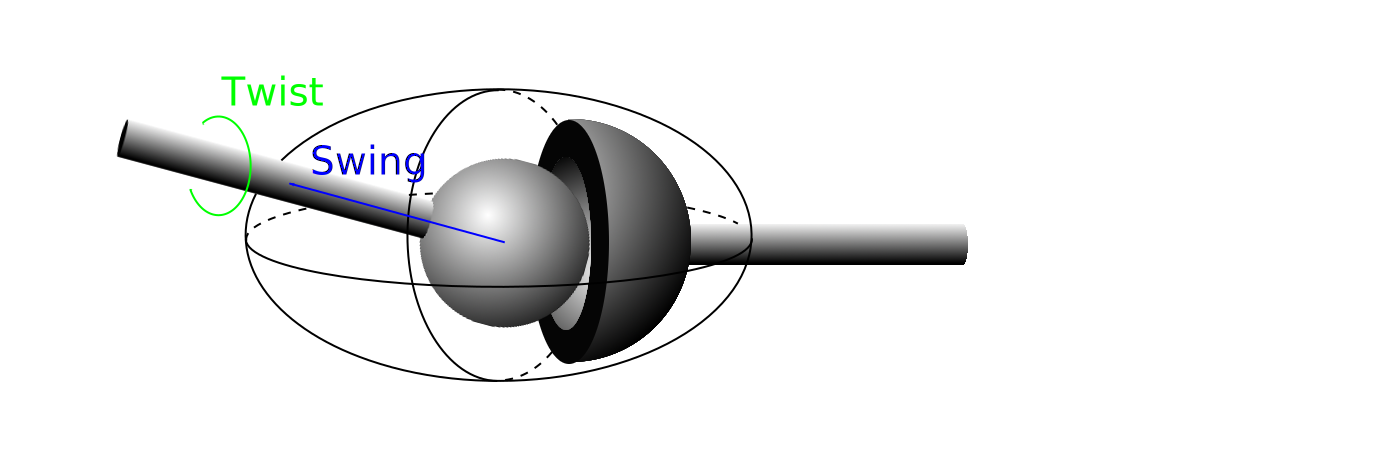
\includegraphics[width=0.7\linewidth]{ballAndSocket.pdf}
  \caption{Swing and Twist in ball and socket joint}
\label{fig:ballAndSocket}
\end{figure}

The spherical motion can be parameterized by a vector of the unit 3D sphere $S2$ and constrained to lay within a limit cone. And the axial motion can be parameterized in $\mathbb{R}$ and be limited by equation~\ref{eq:joint_limits}, this type of formulation is presented in~\cite{baerlocher}.

\subsection{Contact constraints}
\label{sub:contact_constraints}

Humanoid robots evolve in their environment by making and breaking contacts with it.
A contact can be defined between 2 surfaces of different bodies of robots (Note that one of the robots can be the environment or that the two robots can be the same).
The most usual type of contact constraint encountered is the planar contact, where a planar surface of a robot is put in contact with a planar surface of the environment.
We denote $F_1 = \{O_1, \vec{x_1}, \vec{y_1}, \vec{z_1}\}$ a frame defined on $S_1$, the surface of the first body involved in the contact, such that the 3D point $O_1$ is on $S_1$ and the vector $\vec{z_1}$ is normal to $S_1$ and pointing toward the inside the body.
$F2 = \{O_2, \vec{x_2}, \vec{y_2}, \vec{z_2}\}$ is a frame on $S_2$, the surface of the second body involved, such that $O_2$ is on $S_2$ and the vector $\vec{z_2}$ is normal to $S_2$ and pointing away from the body.

Constraining $S_1$ and $S_2$ to be coplanar comes down to aligning $\vec{z_1}$ and $\vec{z_2}$ and to ensure that the projection of the distance between $O_1$ and $O_2$ along $\vec{z_1}$ is null.
Note that we avoid using the dot product of two vectors that are meant to be aligned e.g. $\vec{z_1}\cdot\vec{z_2} = 1$ because when that constraint is satisfied, its gradient is null, which implies that in the optimization context it is unqualified.
That is why we prefer imposing orthogonality constraints.
This translates into adding the following set of constraints to our problem:

\begin{equation}
\label{eq:coplanarity}
\boxed{\left\{
  \begin{array}{l}
    \overrightarrow{O_1O_2} \cdot \vec{z_1} = 0\\
    \vec{x_1}\cdot\vec{z_2} = 0\\
    \vec{y_1}\cdot\vec{z_2} = 0\\
    \vec{z_1}\cdot\vec{z_2} \geq 0
  \end{array}
  \right.}
\end{equation}

This set of constraints leaves free the displacements of $F_2$ along $\vec{x_1}$ and $\vec{y_1}$ as well as its rotation around $\vec{z_1}$.
We call this a floating contact, the optimization algorithm will be able to choose the location of $F_2$ in the plane $\{O_1, \vec{x_1}, \vec{y_1}\}$. This contact has 3 degrees of freedom.

\begin{figure}[htpb]
  \centering
  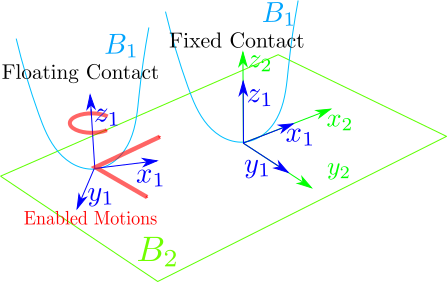
\includegraphics[width=0.8\linewidth]{contactConstraint.pdf}
  \caption{Floating and Fixed Contacts}
\label{fig:contactConstraint}
\end{figure}

If we constrain the location of $F_2$ in $\{O_1, \vec{x_1}, \vec{y_1}\}$ such that $O_1$ and $O_2$ superimposed and $\vec{x_1}$, $\vec{y_1}$, $\vec{z_1}$ are aligned respectively with $\vec{x_2}$, $\vec{y_2}$, $\vec{z_2}$, we obtain a fixed contact with no degree of freedom. This translates into adding the following set of constraints to our problem:

\begin{equation}
\label{eq:fixed_contact}
\boxed{\left\{
  \begin{array}{l}
    \overrightarrow{O_1O_2} = \vec{0}\\
    \vec{x_1}\cdot\vec{z_2} = 0\\
    \vec{y_1}\cdot\vec{z_2} = 0\\
    \vec{x_1}\cdot\vec{y_2} = 0\\
    \vec{z_1}\cdot\vec{z_2} \geq 0\\
    \vec{x_1}\cdot\vec{x_2} \geq 0\\
  \end{array}
  \right.}
\end{equation}

We illustrate those two types of contacts in figure~\ref{fig:contactConstraint}


\subsection{Collision avoidance}
\label{sub:collision_avoidance}

In order to avoid unwanted collisions between bodies of robots, for two bodies $B_1$ and $B_2$, we want to define a continuously differentiable function $d_{\{B_1, B_2\}}(q)$ that has the properties of a pseudo-distance:
\begin{itemize}
  \item $d_{\{B_1, B_2\}}(q) > 0$ when the bodies are not touching each other
  \item $d_{\{B_1, B_2\}}(q) = 0$ when the bodies are in collision without interpenetration
  \item $d_{\{B_1, B_2\}}(q) < 0$ when the bodies are in collision with interpenetration
\end{itemize}

Using the cartesian distance between the exact surfaces of $B_1$ and $B_2$ might result in a discontinuous gradient of $d_{\{B_1, B_2\}}$ if the surfaces of $B_1$ and $B_2$ are not strictly convex.
A conservative approach is to associate to each body, a strictly convex bounding volume and to compute the distance between those volumes.
\cite{escande:humanoids:2007} and~cite{escande:itro:2014} proposes a method to generate a strictly convex Sphere-Torus-Patch Bounding Volumes (STP-BV) that guarantees the gradient continuity of the proximity distance.
The distance between the STP-BV of $B_1$ and $B_2$ computed by an enhanced GJK~\cite{gilbert-1988a} collision-detection algorithm is a continuously differentiable pseudo-distance.
Thus, we can use this function in our optimization algorithm as:

\begin{equation}
  \boxed{d_{\{B_1, B_2\}}(q) > 0}
\end{equation}

This function can be used to avoid collisions between a robot and the environment as well as auto collisions between bodies of the same robot.
We denote $Coll$ the list of triplets $\{B_i, B_j, \epsilon_{ij}\}$ defining each collision that we want to avoid by using this function in our problem, as a pair of bodies $B_i$ and $B_j$ and a minimal distance that we want to keep between them (usually for security reasons).

Then the set of constraints to add to our problem is:

\begin{equation}
  \boxed{\forall \{B_i, B_j, \epsilon_{ij}\} \in Coll,\ d_{\{B_i, B_j\}}(q) > \epsilon_{ij}}
\end{equation}

In many cases, it is possible to avoid the collision between two bodies of a robot by modifying the joint limits and reducing them to a span where the collision of interest cannot happen. That approach is conservative and ad-hoc but can save some precious computation time.

\section{Static constraints}
\label{sec:static_constraints}

\subsection{External Forces}
\label{sub:external_forces}

For a robot to interact with the real world, its geometric description is not enough.
The robot is subject to forces applied on its bodies by the exterior world, those can be generated by contacts with the environment or with another actor (human, another robot, manipulated object\ldots), by the effect of physical forces like gravitation or magnetism, or by contacts between two bodies of the robot.
Our posture generator must take those `External forces' into account, be able to estimate the stability of the robot and compute the internal torques generated in the joints.

An external force applied on a rigid body can also be called a wrench and is composed of a resultant part $f$(sometimes abusively called force) and a moment part (sometimes abusively called couple).
Let $w$ be a wrench, $w|_F^O$ is the expression of $w$ calculated at the point $O$ expressed in the frame $F$.
We denote $\vec{f}$ the resultant part of w, and $\vec{f}|_F$ the expression of $\vec{f}$ in $F$.
$\vec{m}$ is the moment part of $w$ and $\vec{m}|_F^O$ the expression of $\vec{m}$ in $F$ calculated at the point $O$.

\begin{equation}
  w|_F^O = \left\{ \begin{array}{r}
    \vec{m}\\
    \vec{f}\\
  \end{array} \right\}^O_F
  = \left\{ \begin{array}{r}
    \vec{m}|_F^O\\
    \vec{f}|_F\\
  \end{array}\right\}
\end{equation}

The expression of the moment part on a different point $P$ is given by the following formula:

\begin{equation}
  \vec{m}|_F^P = \vec{m}|_F^O + \overrightarrow{PO} \wedge \vec{f}|_F
\end{equation}

Whereas the resultant part is invariant with respect to the point at which the wrench is calculated.

Note that the frame subscript can be dropped in some equations where the choice of the frame does not matter and assuming that all the quantities of the equations are computed in the same frame.

\subsection{Static stability}
\label{sub:static_stability}

We denote $g$ the acceleration of gravity on earth $g = 9.81 m.s^{-2}$.
The wrench associated with the action of gravity on a body of mass $M$ which center of mass is denoted $G$ with $\vec{z}$ the upward vertical vector in the world frame $F_W$ is:
\begin{equation}
  w_g|^G_{F_W} = \left\{ \begin{array}{r}
     \vec{0} \\
     -Mg\vec{z} \\
 \end{array}\right\}^G_{F_W}
\end{equation}

A solid is statically stable if it satisfy the Euler-Newton Equation. We consider a robot on which $m$ external forces $w_i = \left\{ \begin{array}{r}
    \vec{m_i}\\
    \vec{f_i}\\
\end{array} \right\}^{P_i}$ are applied. We denote $P$ the application point on which the equation and all its terms are calculated:
\begin{equation}
  \sum\limits_i w_i|^P + w_g|^P = 0
\end{equation}
Which is equivalent to:
\begin{equation}
\left\{
\begin{array}{r}
  \sum\limits_i \vec{m_i}|^P + \overrightarrow{GP}\wedge Mg\vec{z} = 0 \\
  \sum\limits_i \vec{f_i} - Mg\vec{z} = 0 \\
\end{array}
\right.
\end{equation}

This equation can be simplified by applying it at the center of mass of the body as:
\begin{equation}
  \left\{
  \begin{array}{r}
    \sum\limits_i \vec{m_i}|^G = 0 \\
    \sum\limits_i \vec{f_i} - Mg\vec{z} = 0 \\
  \end{array}
  \right.
\label{eq:stability}
\end{equation}

Satisfying~\ref{eq:stability} ensures the stability of a rigid body.
In some cases, an articulated robot is considered as a rigid body and this equation alone can be used to ensure its stability.
It is only valid if the robot can generate infinite torques in its articulations, or at least if we have some guarantee that the robot is able to generate large enough torques.
Otherwise, it is necessary to verify that the robot's actuators can generate large enough torques to maintain that posture. The details of torque computation are discussed in Section~\ref{sub:torque_limits}

This equation~\ref{eq:stability} can be used in an optimization problem.
We consider that each wrench $w_i$ applied on the system is defined by the position of its application point $P_i$ and the values $m_i$ and $f_i$ that represent the moment and resultant of $w_i$ at $P_i$. $P_i$ depends on $q$ the joint parameter of the robot.
$m_i$ and $f_i$ are new variables that need to be added to the problem. In summary, $w_i$ depends on $q$, $m_i$ and $f_i$.
We denote $f$ the concatenation of all the variables $m_i$ and $f_i$.

\begin{equation}
  \boxed{s(q,f) = \left\{
  \begin{array}{r}
    \sum\limits_i \vec{m_i} + \overrightarrow{P_i G}\wedge \vec{f_i} \\
    \sum\limits_i \vec{f_i} - Mg\vec{z} \\
  \end{array}
  \right\}
  = 0}
\end{equation}

The optimization problem~\ref{eq:optim_form_PG} becomes (we denote m the dimension of the force variables):

\begin{equation}
\label{eq:optim_form_PG_with_stab}
  \left\{
  \begin{array}{l}
    \min\limits_{q\in\mathcal{C}, f\in \mathbb{R}^m}{f(q)}\\
    \text{ s.t. }
    \left\{
    \begin{array}{l}
      s(q,f) = 0\\
      c_i(q) = 0,\ \forall i\in{E}\\
      c_i(q) \geq 0,\ \forall i\in{I}\\
    \end{array}
    \right.
  \end{array}
  \right.
\end{equation}

The derivation of the static stability constraint is straightforward.
All the terms of equation~\ref{eq:stability} are components of wrenches.
A wrench is completely defined by the frame in which it is expressed and its values of resultant and moment in that frame.
Deriving the stability condition comes down to deriving each term w.r.t its components values and w.r.t the transformation of its frame.

\begin{equation}
\left\{
\begin{array}{r}
  \partial\left(\sum\limits_i m_i|^G\right) = \sum\limits_i \partial(m_i|^G) \\
  \partial\left(\sum\limits_i f_i\right) = \sum\limits_i \partial(f_i) \\
\end{array}
\right.
\label{eq:derivation_stability}
\end{equation}

We will explicit a method to automatically compute those derivatives in a further chapter.

\subsection{Center of mass projection}
\label{sub:center_of_mass_projection}

In the case where all the wrenches applied to the body are due to unilateral punctual contacts on points that all lay on the same horizontal plane $H = \{O, \vec{x}, \vec{y}\}$, the stability criterion~\ref{eq:stability} can be simplified.
The wrench $w_i$ generated by a unilateral punctual contact is a pure force resultant, its moment part is null on the contact point.

\begin{equation*}
    \left. w_i \right|^{P_i} =
    \left\{
      \begin{array}{r}
      \vec{0}\\
      \vec{f_i}\\
  \end{array} \right\}^{P_i}
\end{equation*}

\ref{eq:stability} becomes:

\begin{equation}
\left\{
\begin{array}{r}
  \sum\limits_i \overrightarrow{OP_i}\wedge \vec{f_i} - \overrightarrow{OG} \wedge Mg\vec{z} = 0 \\
  \sum\limits_i \vec{f_i} - Mg\vec{z} = 0 \\
\end{array}
\right.
\end{equation}

We can write $\overrightarrow{OG} = \overrightarrow{OG_p} + z_G\vec{z}$ with $G_P$ the projection of $G$ on $H$. Replacing in the moment equation gives:

\begin{equation}
  \sum\limits_i \overrightarrow{OP_i}\wedge \vec{f_i} - \sum\limits_i\overrightarrow{OG_P} \wedge \vec{f_i} = 0
\label{eq:projCoM}
\end{equation}

With $f_i = f_i^x\vec{x} + f_i^y\vec{y} + f_i^z\vec{z}$, $G$ and $P_i$ can be written as $\overrightarrow{OG_P} = G_x \vec{x} + G_y\vec{y}$ and $\overrightarrow{OP_i} = P_{ix} \vec{x} + P_{iy} \vec{y}$. The two first lines of equation~\ref{eq:projCoM} give:

\begin{align}
\sum\limits_i \left\{\begin{array}{r} P_{iy}f_i^z\\-P_{ix}f_i^z\end{array}\right\}
= \left\{\begin{array}{r} G_{y}\\-G_{x}\end{array}\right\} \sum\limits_i f_i^z\\
  \overrightarrow{OG_P} = \frac{\sum\limits_i \overrightarrow{OP_i} f_i^z}{\sum\limits_i f_i^z}
\end{align}

Since all the contacts are unilateral on the same plane, all the $f_i^z$ are positive.
For any set of $f_i^z\geq0$, $G_P$ is a barycenter with positive coefficients of the set of all $P_i$.
Any point $G_P$ that is included in the convex hull of all the $P_i$ is a solution.

Thus, we have the property: A rigid body that has all its contacts with the environment being punctual, unilateral and all laying on the same horizontal plane $H$ is stable if and only if the projection of its center of mass on $H$ is inside the convex hull of all its contact points.

\subsection{Torque limits}
\label{sub:torque_limits}

In general, satisfying equation~\ref{eq:stability} is not enough to ensure that a robot can be statically stable.
The joint torques that are required to hold the posture must be within the physical capabilities of the robot, namely, its torque limits.
We denote $\tau_i^-$ and $\tau_i^+$ the minimal and maximal torques that can be generated by the robot's actuators on joint $J_i$.
Note that in some cases, the torque limits are not constant and can depend on the joint parameters $\tau_i^-(q)$ and $\tau_i^+(q)$.
For example, it is the case with the Atlas robot that is hydraulically actuated.

Featherstone~\cite{featherstone:book:2007} proposes a recursive algorithm to compute the torques, accelerations, and velocities generated in a multi-articulated system by a set of external forces called the Inverse Dynamics Algorithm.
For the purpose of generating statically stable postures, the velocities and accelerations are useless.
Thus, we devise a specialized algorithm to fit our needs and call it the Inverse Static Algorithm.

The algorithm first computes the generalized forces $f^G_i$ applied to each body, it is the sum of the action of gravity and of the external forces applied on a body calculated at the origin of the world frame, expressed in the world frame.
Then, the generalized forces are used to compute the torques.

\begin{algorithm}
  \caption{Inverse Static Algorithm}
\label{IS}
\begin{algorithmic}
  \For{$i = 0:n_B$}
  \State$f^G_i = \mathbf{I}^W {}^i\mathbf{X}_W \mathbf{a}^G - {{}^i\mathbf{X}_W}^*f_i^{ext}$
  \EndFor{}
  \For{$i = n_J-1:0$}
  \State$\tau_i = {f^G_i}^T S_i$
  \If{$pred(i) \neq -1$}
  \State$f^G_{pred(i)} += {\mathbf{X}^{PtS}_i(q)}^{-*} f^G_i$
  \EndIf{}
  \EndFor{}
\end{algorithmic}
\end{algorithm}

We can write the torques as a function of the joint parameters and the external forces $\tau(q,f)$.
The torque limit constraint writes as:
\begin{equation}
  \boxed{\tau^- \leq \tau(q,f) \leq \tau^+}
\end{equation}

We will detail the derivation of this constraint in a further chapter.

\subsection{Contact Forces and Friction Cones}

Here we use the same frames and notations as introduced in Section~\ref{sub:contact_constraints}.

The contacts involved in a posture generation problem can be separated into two types: Geometric Contacts and Stability Contacts.

The Geometric Contact is a contact without forces, the two bodies are touching each other, but do not apply any force on each other.
Physically, that correspond to the transition state between a configuration without contact and a configuration with contact on which forces are applied.
We defined the Geometric Contacts in Section~\ref{sub:contact_constraints}.
The Stability Contact is a Geometric Contact that bears interaction forces.
We denote $w_{1\rightarrow 2}$ the force applied by body $B_1$ on body $B_2$. Then the force applied by $B_2$ on $B_1$ is $w_{2\rightarrow 1} = -w_{1\rightarrow 2}$.
These interaction forces must be taken into account in the stability and torque computations of each robot involved in the contact.

The interaction force resulting from a punctual contact (see figure~\ref{fig:frictionCone}) on a point $P$ can be modeled as a pure force resultant along the $z_1$ direction $\vec{f_n} = f_z \vec{z_1}$ and the tangential efforts due to the friction in that contact can be modeled as $\vec{f_t} = f_x \vec{x_1} + f_y \vec{y_1}$. A punctual contact cannot carry moments on its contact point.

\begin{equation}
\label{eq:punctual_force}
\left. w_{2\rightarrow 1}\right|^P = \left\{
  \begin{array}{l}
    \vec{0} \\
    \overrightarrow{f_{2\rightarrow 1}} = \vec{f_t} + \vec{f_n} \\
  \end{array}
  \right\}^P
\end{equation}

\begin{figure}[htpb]
  \centering
  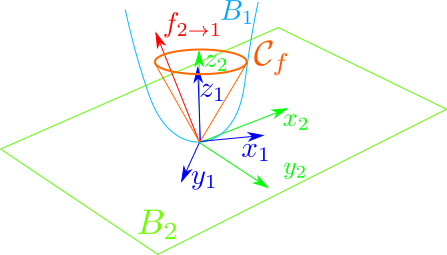
\includegraphics[width=0.6\linewidth]{frictionCone.pdf}
  \caption{Punctual unilateral Stability contact with friction}
\label{fig:frictionCone}
\end{figure}

This formulation of the interaction force defines a bilateral contact, in the sense that the force can be in any direction, $B_1$ can push as well as pull on $B_2$.

To model a unilateral contact, we must constrain the normal component of $f_{2\rightarrow 1}$ to be oriented toward the inside of $B_1$. Which means that only pushing actions can be generated, not pulling actions.
This translates into:
\begin{equation}
  \overrightarrow{f_{2\rightarrow 1}}\cdot \vec{z_1} = f_z \geq 0
\end{equation}

Furthermore, for the contact to be stable, the Coulomb friction law must be respected.
This law states that the contact force resultant must lay inside a friction cone of angle $\mu$, the friction coefficient.
Which translates into the following equation:

\begin{equation}
  \mu\|\vec{f_n}\| \geq \|\vec{f_t}\|
\end{equation}

Given the decomposition of $f_{2\rightarrow 1}$ in $F_1$, $f_{2\rightarrow 1} = f_x \vec{x_1} + f_y \vec{y_1} + f_z \vec{z_1}$.
For any punctual contact in a posture generation problem, we can add the following set of constraint to our optimization problem:

\begin{equation}
  \label{eq:unilateralContact}
  \left\{
  \begin{array}{l}
    f_z \geq 0 \\
    \mu^2 f_z^2 - f_x^2 +f_y^2 \geq 0
  \end{array}
  \right.
\end{equation}

When it comes to planar contacts on surface $S$ with $\vec{n}$ the outbound normal to $S$, the interaction force can have components of forces and moments in all directions.
The forces components intrinsic to the planar contact model are a resultant part aligned with $\vec{n}$ $\vec{f_n} = f_z \vec{z_1}$ and a moment part tangential to $S$: $\vec{m_t} = m_x \vec{x_1} + m_y \vec{y_1}$.
The forces due to friction are a tangential friction resultant part $\vec{f_t} = f_x \vec{x_1} + f_y \vec{y_1}$ and a normal friction moment $\vec{m_n} = m_z \vec{z_1}$.

This type of force can be modeled by a set of unilateral punctual efforts applied on each vertex of a polygon describing the contact area.
And ensuring that each of them lay in their respective friction cone, thus satisfying the equation~\ref{eq:unilateralContact}. As depicted in figure~\ref{fig:planarContact}

\begin{figure}[htpb]
  \centering
  \setlength{\fboxsep}{0pt}%
  \setlength{\fboxrule}{1pt}%
  \fbox{\includegraphics[width=0.6\linewidth]{planarContact.pdf}}
  \caption{Modelization of a Planar Contact between the foot on HRP4 and the ground}
\label{fig:planarContact}
\end{figure}

\section{Cost Functions}
\label{sec:cost_functions}

In addition to constraints, it is often useful to add a cost function to our optimization problem.
The submanifold of feasible configurations $\mathcal{C}_F$ can contain an infinity of solutions and even some continuous solution areas in which all points are solutions.
The cost function helps to choose the "best" candidate solution.
Various types of cost functions can be chosen, for example, we can minimize the distance to a reference posture $q_R$:

\begin{equation*}
  f_\text{posture}(q) = \|q-q_R\|
\end{equation*}

The effect of that type of cost function is illustrated in figure~\ref{fig:cost}. On both images, the HRP-2 Kai robot is stable, respects its joints and torques limits. The only difference is that the right one mimimizes the distance to a reference posture (standing straight with bent knees) while the left result does not use a cost function.

\begin{figure}[htpb]
  \centering
  \setlength{\fboxsep}{0pt}%
  \setlength{\fboxrule}{1pt}%
  \fbox{\includegraphics[width=0.5\linewidth]{cost.pdf}}
  \caption{Effect of cost function. Left: no cost function. Right: Distance to posture}
  \label{fig:cost}
\end{figure}

We can also want to minimize the sum of norms of contact forces:
\begin{equation*}
  f_\text{forces}(f) = \sum\limits_i \|f_i(f)\|
\end{equation*}
Or the torques in the robot's joints:
\begin{equation*}
  f_\text{torques}(q,f) = \sum\limits_i \|\tau_i(q,f)\|
\end{equation*}
Some more custom cost functions can also be considered, for example, we can want a point $P_i$ on body $B_i$ with to be as far as possible in a direction $\vec{d}$
\begin{equation*}
  f_\text{point} (q) = -{\overrightarrow{O_W P_i}}\cdot{\vec{d}}
\end{equation*}

Any positively weighted combination of cost function can be used. In which case it is important to choose the weights carefully to scale all the costs so that they all can influence the result and none is completely dominated by another.
\begin{equation}
  f_\text{cost}(q,f) = \sum\limits_i{w_if_i(q,f)} = w_0 f_\text{posture}(q) + w_1 f_\text{forces}(f) + w_2f_\text{torques}(q,f) + \cdots
\end{equation}

\section{Conclusion}
\label{sec:Ch1_Conclusion}

In this section, we have seen how to formulate a robotics problem with several different tasks and objectives as an optimization problem.

We denote $\mathcal{T}_i$ the additional tasks added to the problem, which is described by the set of equations $g_i(q,f) = 0$ and inequations $h_i(q,f) \geq 0$.
The contact tasks are included in those and the equations describing them must encompass the geometric contact constraint equation like~\ref{eq:coplanarity} as well as the unilaterality and friction equations~\ref{eq:unilateralContact} in the case of a unilateral contact.

A typical robotics problem can be written as a combination of all those costs and constraints:
\begin{align}
\min_{q, f} & \quad f_\text{cost}(q,f) \nonumber\\
\text{s.t.}&
\left\{
\begin{array}{lr}
q^- \le q \le q^+\\
s(q,f) = 0 \\
\tau^- \le \tau(f,q) \le \tau^+\\
\forall \{B_i, B_j, \epsilon_{ij}\} \in Coll,\ d_{\{B_i, B_j\}}(q) > \epsilon_{ij}\\
g_i(q,f) = 0\ \ \forall\mathcal{T}_i,\\
h_i(q,f) \geq 0\ \ \forall\mathcal{T}_i.
\end{array}\right.
\label{eq:PG}
\end{align}




